\chapter{Dynamic Expansion}
In this chapter, we describe further why we introduce \tdynexp, and present how we design this feature. After that, we describe how to construct \tsieve in \tdynexp and finally present the problem we encounter during implementing \tdynexp.

We described \tsieve in the Use Cases chapter and it is our main motivation to allow developers to construct workflows like that more naturally and universally. By introducing \tdynexp, we expect to allow developers to design \tPETmpl{}s which are elastic according to actual needs while keeping backward compatibilities with the existing \dpy mechanism.

\section{PE Definition} \label{sec:dynexp_PE_def}
To introduce the dynamics, we need to add some extra mechanisms to the definition of PEs (\ie \tPETmpl{}s). We now present the general need, followed by our implementation.

In general, each PE should decide whether to \textit{expand} or not when receiving and processing data. We use the term \textit{expand} to limit this dynamics to a handleable range or the range will explode. By saying \textit{expand}, we expect each PE behave like cell division, to split to another almost the same PE, when the mechanism is triggered, and we limit this mechanism to trigger at most once for each expandable condition each PE (and the divisional PE will be treated as if it is a PE defined in the workflow so it can still \textit{expand}).

Although we limit this mechanism to \textit{expand} for our prototype system, it is capable to accomplish the design of \ttsieve as well as other workflows containing a similar behaviour. Moreover, by combining the expansion behaviour with the mechanism used to bundle multiple PEs together to form a large PE (which is an unnamed mechanism in \dpy), developers can design more complex expansion behaviours.

In the above discussion, we deliberately blurred the difference between \tPETmpl and \tPEInst for simplicity, and we believe this won't cause confusion for readers.

To implement \tdynexp, we add two more features to the definition of each PE (\tPETmpl):

\defTerm{circuit}{circuit}

\begin{enumerate}
	\item A \textbf{property} used to inform the coordinator (and the developer) whether this PE (\tPETmpl) is expandable or not. \\
	This is implemented as a read-only property called \lstinline|repeatable| in the definition of PE, and defaults to \lstinline|False|. The developer only needs to override this property to \lstinline|True| when designing an expandable PE.
	\item A \textbf{mechanism} used to control when to trigger the expansion and how to communicate to the expanded PE. \\
	We add a special type of output connections called ``\tcircuit''. Each \tcircuit is a pair of connections (one input and one output), both defined in the same \tPETmpl. When the PE sends data through an output connection defined in the \tcircuit, the expansion mechanism is trigger, a division is deployed and the data is sent to the paired input connection in the \tcircuit. This \tcircuit then becomes a static connection, meaning this (old) PE can keep sending more data through this output connection and no more division will be triggered.
\end{enumerate}

\section{Runtime Behaviour}
The section above described how \tdynexp is designed in the PE part, and briefly mentioned the meaning of each of these features. This section describe how these features are expected to work during runtime, and then describe it in our implementation, mainly from the perspective of the coordinator.

An expandable PE (\emph{origin}) sends sends a signal containing the \tcircuit output connection. The system recognizes this is a request for expansion, prepares the divisional PE (which is almost a ``duplication'' to the PE (\emph{origin}), with extra configurations) and deploy the divisional PE so the \emph{origin} can subsequently communicate with the divisional PE.

Our implementation builds on top of \tincdep, and utilize many of its features. In our implementation, an expandable PE outputs data through a \tcircuit output connection using the same way as other output connections -- sending a signal to the coordinator. The coordinator checks if the PE(\emph{origin} is expandable, and then checks if the output connection is an output connection defined in \tcircuit. If both true, the coordinator will create a duplication to the PE (\emph{origin}), and deploy it to a node, using the same way as a common \tincdep.

To avoid confusion, when sending the ID of PE to a node during deployment, the divisional PE will contain a separate field with an increasing integer count. When the node receives this message, it extracts the PE ID part to obtain the PE, and ignores the other part (\ie the counter) in the current implementation.

\section{Simple Example} \label{sec:dynexp_example}
In this section, we use \ttsieve as our example to show the difference of the semantics before and after implementing \tdynexp.

We have described the structure of \ttsieve in \ref{sec:uc_sieve} (see also Figure \ref{fig:sieve_static}). If we want to construct it in the original version of \dpy, we need to estimate the number of sieves to construct the workflow. For example, if we want to know the primes up to 100, we need to assign at least 26 sieve PEs. Listing \ref{lst:wf_sieve} gives an example code to construct this workflow.

\begin{figure}[h]\centering
    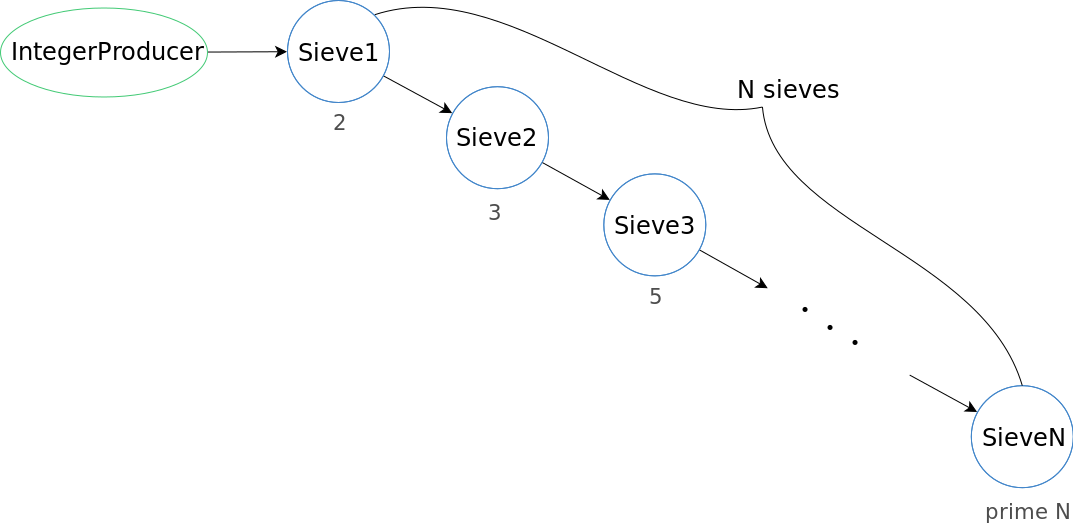
\includegraphics[width=0.8\textwidth]{figures/sieve_static}
	\caption{Workflow for the prime sieve}	\label{fig:sieve_static}
\end{figure}

\begin{lstlisting}[frame=single,caption={Example code of the sieve workflow construction in the old semantics (suppose IntegerProducer and PrimeSieve are already defined},captionpos=b,label={lst:wf_sieve}]
from dispel4py.workflow_graph import WorkflowGraph

producer = IntegerProducer(2, 100)
sieve = PrimeSieve()
graph = WorkflowGraph()
graph.connect(producer, 'output',
              sieve, PrimeSieve.INPUT_NUMBER)

prev = sieve
for i in range(1, 26):
    sieve = PrimeSieve()
    graph.connect(prev, PrimeSieve.OUTPUT_NUMBER,
                  sieve, PrimeSieve.INPUT_NUMBER)
    prev = sieve
\end{lstlisting}

It is also legal and correct to construct this workflow with sieves more than enough. For example, we can change the number 26 in line 10 to a larger number, say, 100. This workflow can also be executed and correct result will be gathered. The only problem is more nodes are needed to run this workflow, even if some nodes are actually unused (\ie no data will be sent to these nodes).

The problem in this approach is that the number of sieves is unknown in the nature of this algorithm, but the number is required to define the workflow. As discussed in \ref{sec:uc_sieve}, we encounter a chicken-and-egg problem. This problem also makes the workflow not universal because the number of sieve PEs is different for different ranges of numbers.

In \tdynexp, we introduce the expansion behaviour so this problem is eliminated. To construct such a workflow, we only need to create a expandable sieve PE, and add it only once to the workflow. Example code is shown in Listing \ref{lst:wf_sieve_dynexp}.

\begin{lstlisting}[frame=single,caption={Example code of the sieve workflow construction in the new semantics (suppose IntegerProducer and ExpandablePrimeSieve are already defined},captionpos=b,
label={lst:wf_sieve_dynexp}
]
from dispel4py.workflow_graph import WorkflowGraph

producer = IntegerProducer(2, 100)
sieve = ExpandablePrimeSieve()
graph = WorkflowGraph()
graph.connect(producer, 'output',
              sieve, ExpandablePrimeSieve.INPUT_NUMBER_LINE)
\end{lstlisting}

Our definition to the \lstinline|ExpandablePrimeSieve| is shown in Listing \ref{lst:wf_sieve_PE_def}). This definition mainly serves the purpose of illustrating usage, rather than performance.

\begin{lstlisting}[frame=single,caption={Example code of the ExpandablePrimeSieve class},captionpos=b,
label={lst:wf_sieve_PE_def}
]
class ExpandablePrimeSieve(RepeatablePE):
    INPUT_NUMBER_LINE = 'input'
    OUTPUT_NUMBER_LINE = 'output'
    OUTPUT_NUMBER = 'number'

    def __init__(self):
        super(ExpandablePrimeSieve, self).__init__()
        self.number = None
        self._add_input(ExpandablePrimeSieve.INPUT_NUMBER_LINE)
        self._add_output(ExpandablePrimeSieve.OUTPUT_NUMBER_LINE)
        self._add_output(ExpandablePrimeSieve.OUTPUT_NUMBER)
        self._add_circuit(ExpandablePrimeSieve.OUTPUT_NUMBER_LINE,
                          ExpandablePrimeSieve.INPUT_NUMBER_LINE)

    def _preprocess(self):
        self.number = None

    def process(self, inputs):
        number = inputs[ExpandablePrimeSieve.INPUT_NUMBER_LINE]
        if self.number is None:
            self.number = number
            outputs = {ExpandablePrimeSieve.OUTPUT_NUMBER: number}
        else:
            if number % self.number != 0:
                outputs = {ExpandablePrimeSieve.OUTPUT_NUMBER_LINE: number}
            else:
                outputs = None
\end{lstlisting}

Notice the \lstinline|ExpandablePrimeSieve| inherits from \lstinline|RepeatablePE| rather than a common \lstinline|GenericPE| (or other subclasses of it). \lstinline|RepeatablePE| is a special subclass of \lstinline|GenericPE| supporting the \tdynexp features. It defines itself expandable (by setting the \lstinline|repeatable| property to \lstinline|True|) and adds the functionalities to add circuits (both briefly discussed in \ref{sec:dynexp_PE_def}). Example code is shown in Listing \ref{lst:wf_RepeatablePE_def}.

\begin{lstlisting}[frame=single,caption={Example code of the ExpandablePrimeSieve class},captionpos=b,
label={lst:wf_RepeatablePE_def}
]
class RepeatablePE(GenericPE):
    def __init__(self, numprocesses=1):
        super(RepeatablePE, self).__init__(numprocesses)
        self._circuit = {}

    @property
    def repeatable(self):
        return True

    def _add_circuit(self, output_name, input_name):
        try:
            self._circuit[output_name].append(input_name)
        except KeyError:
            self._circuit[output_name] = [input_name]

    def get_circuit(self, output_name):
        try:
            return list(self._circuit[output_name])
        except KeyError:
            return []

    def get_circuit_outputs(self):
        return list(self._circuit.keys())
\end{lstlisting}

Using these definitions, the workflow in the new semantics is more universal than that in the old semantics. Although it seems the \lstinline|IntegerProducer| still needs to be changed when changing the maximum number, this is indeed the issue of our implementation choice -- instead of a PE with a pre-defined range, we can use a producer PE which reads from commandline arguments or a file to get the number range. We use this pre-defined kind of PEs here in order to better present the design and meaning of the workflow.
